
\documentclass[
a4paper,     %% defines the paper size: a4paper (default), a5paper, letterpaper, ...
% landscape,   %% sets the orientation to landscape
% twoside,     %% changes to a two-page-layout (alternatively: oneside)
% twocolumn,   %% changes to a two-column-layout
 headsepline, %% add a horizontal line below the column title
footsepline, %% add a horizontal line above the page footer
titlepage,   %% only the titlepage (using titlepage-environment) appears on the first page (alternatively: notitlepage)
 halfparskip,     %% insert an empty line between two paragraphs (alternatively: halfparskip, ...)
% leqno,       %% equation numbers left (instead of right)
 fleqn,       %% equation left-justified (instead of centered)
% tablecaptionabove, %% captions of tables are above the tables (alternatively: tablecaptionbelow)
% draft,       %% produce only a draft version (mark lines that need manual edition and don't show graphics)
% 10pt         %% set default font size to 10 point
% 11pt         %% set default font size to 11 point
12pt         %% set default font size to 12 point
]{scrartcl}  %% article, see KOMA documentation (scrguide.dvi)



%%%%%%%%%%%%%%%%%%%%%%%%%%%%%%%%%%%%%%%%%%%%%%%%%%%%%%%%%%%%%%%%%%%%%%%%%%%%%%%%
%%%
%%% packages
%%%

%%%
%%% encoding and language set
%%%

%%% ngerman: language set to new-german
\usepackage{ngerman}

%%% babel: language set (can cause some conflicts with package ngerman)
%%%        use it only for multi-language documents or non-german ones
\usepackage[ngerman]{babel}

%%% inputenc: coding of german special characters
\usepackage[utf8]{inputenc}

%%% fontenc, ae, aecompl: coding of characters in PDF documents
\usepackage[T1]{fontenc}
\usepackage{ae,aecompl}

%%%
%%% technical packages
%%%

\usepackage{multirow}

%%% amsmath, amssymb, amstext: support for mathematics
\usepackage{amsmath,amssymb,amstext}

%%% psfrag: replace PostScript fonts
%\usepackage{psfrag}

%%% listings: include programming code
\usepackage{listings}

%%% units: technical units
\usepackage{units}

%%%
%%% layout
%%%

%%% scrpage2: KOMA heading and footer
%%% Note: if you don't use this package, please remove 
%%%       \pagestyle{scrheadings} and corresponding settings
%%%       below too.
\usepackage{scrpage2}

%%%
%%% PDF
%%%

\newif\ifpdf
  \ifx\pdfoutput\undefined
     \pdffalse
  \else
     \pdfoutput=1
     \pdftrue
  \fi

%%% Should be LAST usepackage-call!
%%% For docu on that, see reference on package ``hyperref''
\ifpdfoutput{%   (definitions for using pdflatex instead of latex)

  %%% graphicx: support for graphics
  \usepackage[pdftex]{graphicx}

  \pdfcompresslevel=9

  %%% hyperref (hyperlinks in PDF): for more options or more detailed
  %%%          explanations, see the documentation of the hyperref-package
  \usepackage[%
    %%% general options
    pdftex=true,      %% sets up hyperref for use with the pdftex program
    %plainpages=false, %% set it to false, if pdflatex complains: ``destination with same identifier already exists''
    %
    %%% extension options
    backref=true,      %% if true, adds a backlink text to the end of each item in the bibliography
    pagebackref=false, %% if true, creates backward references as a list of page numbers in the bibliography
    colorlinks=false,   %% turn on colored links (true is better for on-screen reading, false is better for printout versions)
    %
    %%% PDF-specific display options
    bookmarks=true,          %% if true, generate PDF bookmarks (requires two passes of pdflatex)
    bookmarksopen=false,     %% if true, show all PDF bookmarks expanded
    bookmarksnumbered=false, %% if true, add the section numbers to the bookmarks
    %pdfstartpage={1},        %% determines, on which page the PDF file is opened
    pdfpagemode=None         %% None, UseOutlines (=show bookmarks), UseThumbs (show thumbnails), FullScreen
  ]{hyperref}


  %%% provide all graphics (also) in this format, so you don't have
  %%% to add the file extensions to the \includegraphics-command
  %%% and/or you don't have to distinguish between generating
  %%% dvi/ps (through latex) and pdf (through pdflatex)
  \DeclareGraphicsExtensions{.pdf}

}{%else   (definitions for using latex instead of pdflatex)

  \usepackage[dvips]{graphicx}

  \DeclareGraphicsExtensions{.eps}

  \usepackage[%
    dvips,           %% sets up hyperref for use with the dvips driver
    colorlinks=false %% better for printout version; almost every hyperref-extension is eliminated by using dvips
  ]{hyperref}

}


%%% sets the PDF-Informations options
%%% (see fields in Acrobat Reader: ``File -> Document properties -> Summary'')
%%% Note: this method is better than as options of the hyperref-package (options are expanded correctly)
\hypersetup{
  pdftitle={Einrichtung einer internen Firewall von Firma-a und Firma-b und LAN-to-LAN-VPN Firma-a	(Server)	
nach	 Firma-b(Client)}, %%
  pdfauthor={}, %%
  pdfsubject={IT Sicherheitsarchitekturen}, %%
  pdfcreator={Accomplished with LaTeX2e and pdfLaTeX with hyperref-package.}, %% 
  pdfproducer={}, %%
  pdfkeywords={} %%
}


%%%%%%%%%%%%%%%%%%%%%%%%%%%%%%%%%%%%%%%%%%%%%%%%%%%%%%%%%%%%%%%%%%%%%%%%%%%%%%%%
%%%
%%% user defined commands
%%%

%%% \mygraphics{}{}{}
%% usage:   \mygraphics{width}{filename_without_extension}{caption}
%% example: \mygraphics{0.7\textwidth}{rolling_grandma}{This is my grandmother on inlinescates}
%% requires: package graphicx
%% provides: including centered pictures/graphics with a boldfaced caption below
%% 
\newcommand{\mygraphics}[3]{
  \begin{center}
    \includegraphics[width=#1, keepaspectratio=true]{#2} \\
    \textbf{#3}
  \end{center}
}

%%%%%%%%%%%%%%%%%%%%%%%%%%%%%%%%%%%%%%%%%%%%%%%%%%%%%%%%%%%%%%%%%%%%%%%%%%%%%%%%
%%%
%%% define the titlepage
%%%

 \subject{IT Sicherachitekturen}   %% subject which appears above titlehead
% \titlehead{} %% special heading for the titlepage

%%% title
\title{Einrichtung einer internen Firewall von Firma-a und Firma-b, sowie LAN-to-LAN-VPN von Firma-a (Server)	
nach	 Firma-b(Client)}

%%% author(s)
\author{Paul Drautzburg \and
Georg Mohr}

%%% date
\date{HTWG Konstanz, Sommersemester 2018}

% \publishers{}

% \thanks{} %% use it instead of footnotes (only on titlepage)

% \dedication{} %% generates a dedication-page after titlepage


%%% uncomment following lines, if you want to:
%%% reuse the maketitle-entries for hyperref-setup
%\newcommand\org@maketitle{}
%\let\org@maketitle\maketitle
%\def\maketitle{%
%  \hypersetup{
%    pdftitle={\@title},
%    pdfauthor={\@author}
%    pdfsubject={\@subject}
%  }%
%  \org@maketitle
%}


%%%%%%%%%%%%%%%%%%%%%%%%%%%%%%%%%%%%%%%%%%%%%%%%%%%%%%%%%%%%%%%%%%%%%%%%%%%%%%%%
%%%
%%% set heading and footer
%%%

%%% scrheadings default: 
%%%      footer - middle: page number
\pagestyle{scrheadings}

%%% user specific
%%% usage:
%%% \position[heading/footer for the titlepage]{heading/footer for the rest of the document}

%%% heading - left
% \ihead[]{}

%%% heading - center
% \chead[]{}

%%% heading - right
 %\ohead[]{}

%%% footer - left
% \ifoot[]{}

%%% footer - center
% \cfoot[]{}

%%% footer - right
% \ofoot[]{}



%%%%%%%%%%%%%%%%%%%%%%%%%%%%%%%%%%%%%%%%%%%%%%%%%%%%%%%%%%%%%%%%%%%%%%%%%%%%%%%%
%%%
%%% begin document
%%%

\begin{document}

 \pagenumbering{roman} %% small roman page numbers

%%% include the title
% \thispagestyle{empty}  %% no header/footer (only) on this page
 \maketitle

%%% start a new page and display the table of contents
 \newpage
 \tableofcontents

%%% start a new page and display the list of figures
 \newpage
 \listoffigures

%%% start a new page and display the list of tables
\newpage
 \listoftables

%%% display the main document on a new page 
 \newpage

 \pagenumbering{arabic} %% normal page numbers (include it, if roman was used above)

%%%%%%%%%%%%%%%%%%%%%%%%%%%%%%%%%%%%%%%%%%%%%%%%%%%%%%%%%%%%%%%%%%%%%%%%%%%%%%%%
%%%
%%% begin main document
%%% structure: \section \subsection \subsubsection \paragraph \subparagraph
%%%

\section{Motivation}
Im Zeitalter der Digitalisierung steigt der Grad der Vernetzung immer weiter an. Unternehmen, die ihre Standorte über die ganze Welt verteilt haben, wollen Wege und Möglichkeiten haben ihre Arbeit sicher und problemlos zu verrichten. Dafür ist es unerlässlich, dass verschiedene Standorte auf Ressourcen des Anderen zugreifen können. Für solche Szenarien gibt es in der Netzwerktechnik und Netzwerkarchitektur verschiedene Lösungsansätze. 
Jedoch darf dabei ein wichtiger Aspekt nicht vernachlässigt werden, denn jedes Unternehmen hat Betriebsmittel und Informationen, welche keiner Gefahr von Außen ausgesetzt werden sollen. An diesem Punkt kommt der Begriff IT-Sicherheit ins Spiel und genau dieses Umfeld, um den Begriff "IT-Sicherheit“, wird im Rahmen des Praktikums zur Lehrveranstaltung "IT-Sicherheitsarchitekturen“ untersucht. 
In den folgenden Kapiteln wird eine Problemstellung unter Laborbedingungen skizziert, welche ein Szenario widerspiegelt, mit dem sich Unternehmen täglich konfrontiert sehen. Anschließend werden die Laborbedingungen und der Versuchsaufbau beschrieben. Aus der Problemstellung und dem Versuchsaufbau wird eine Lösung auf Grundlage des theoretischen Hintergrunds erarbeitet. Diese Lösung wird abschließend in die Laborumgebung implementiert und auf ihre Akzeptanz gegenüber der Problemstellung untersucht und in einem Fazit bewertet.   
\newpage
\section{Problemstellung}
In diesem Kapitel wird die Laborumgebung eingeführt und beschrieben, sowie die damit verbundene Aufgaben- und Problemstellung skizziert.
\subsection{Laborumgebung und Versuchsaufbau}
\label{laborumgebung}
Im Labor wird die IT-Landschaft zweier Unternehmen "A“ und "B“ simuliert. Jedes Unternehmen besitzt ein lokales LAN, an denen die potentiellen Mitarbeiter angeschlossen sind. Zudem gibt es mehrere Server, mit  deren Hilfe verschiedene Dienste angeboten werden sollen. 
Diese Dienste werden nachfolgend aufgelistet:

\begin{itemize}
\item Internetzugang von den Mitarbeiter-Computern,
\item Zugang über HTTPS der Webseiten beider Unternehmen,
\item Eine virtuelle Kopplung der beiden Unternehmen mit Hilfe einer sog. Site-to-Site Verbindung,
\item Jeder Mitarbeiter der Unternehmen, soll die Möglichkeit haben, E-Mails über einen sicheren  Mailserver zu verschicken.
\end{itemize}
Eine weitere wichtige Komponente in dieser IT-Landschaft sind die externen und internen Firewalls, da diese den Grundstein für eine sichere Umgebung legen. In dieser IT-Landschaft gibt es insgesamt vier Firewalls, jedes Unternehmen hat jeweils eine interne und externe Firewall. Hinter den externen Firewalls der Unternehmen liegt die sogenannte DMZ – Demilitarisierte Zone. In dieser Zone stehen üblicherweise die Unternehmensserver, welche nach außen hin von der externen Firewall und nach innen von der internen Firewall geschützt werden. Jede Firewall läuft auf einem Server und somit besteht die IT-Landschaft insgesamt aus vier Servern, auf welchen die Firewalls laufen, zwei Servern, welche die jeweiligen Unternehmensserver simulieren und einem Server welcher außerhalb der externen Firewall das Internet simulieren soll (vgl. Abb. \ref{fig:appStat}).

\begin{figure}[!h]
	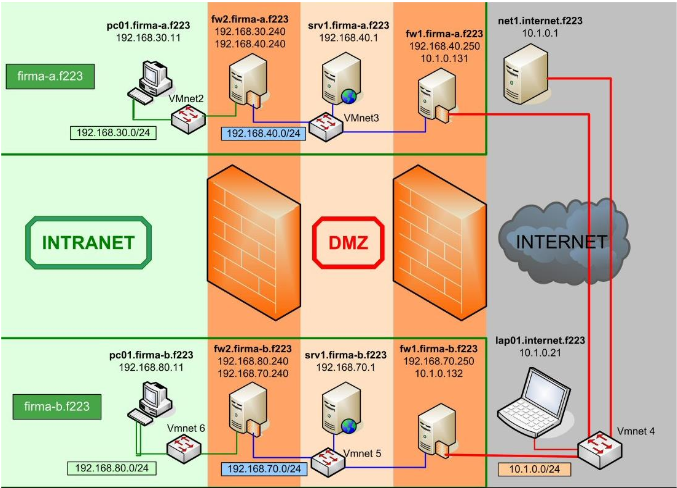
\includegraphics[width=\textwidth]{pictures/laborumgebung.png}
	\caption{Schematischer Aufbau der Laborumgebung im IT-Sicherheitslabor \cite{JueNeuSaDue}}
	\label{fig:appStat}
\end{figure}

Jede dieser angesprochenen Komponenten muss entsprechen konfiguriert werden, damit die angesprochenen Dienste fehlerfrei funktionieren können.
Technisch gesehen wird jeder dieser Server auf Grundlage einer virtuellen Maschine abgebildet.
Auf jeder dieser Maschinen ist Linux als Betriebssystem installiert und vorkonfiguriert, jedoch ohne zusätzliche Pakete, nur die reine Grundinstallation. Da die Implementierung und Installation all dieser Dienste und der damit verbundenen Komponenten, den Rahmen dieses Praktikums sprengen würden, wird die Aufgabenstellungen runter gebrochen. Die detaillierte Aufgabenstellung wird im nächsten Abschnitt eingeführt.

\subsection{Aufgabenstellung}\label{kap:Aufgabenstellung}
Wie schon im vorhergehenden Abschnitt beschrieben, gibt es mehrere Dienste, welche in der IT-Landschaft angeboten werden sollen. 
In diesem Bericht wird die Virtuelle Kopplung der Unternehmen "A“ und "B“ durch eine "Site-to-Site-“, oder auch "LAN-to-LAN-“ genannt, Verbindung implementiert. 
Die Problemstellung gilt als gelöst, wenn es möglich ist, dass das Unternehmen "A" eine gesicherte Verbindung zu Unternehmen "B" aufbauen kann und die jeweiligen internen Firewalls entsprechend konfiguriert sind. Die Konfiguration der externen Firewalls kann in dieser Aufgabe vernachlässigt werden, hierfür sollen die bereitgestellten Firewalls verwendet werden. 

\section{Theoretische Grundlagen}
In diesem Kapitel werden die theoretischen Grundlagen eingeführt, welche im Kontext der Aufgabestellung benötigt werden. Dies beschränkt sich auf fünf Bereiche: die Netzwerkarchitekturen, Debian GNU Linux 7.11, IP-Tables, PKI und OpenVPN. Jede dieser genannten Bereiche wird innerhalb dieses Kapitels eingeführt und in den Aufgabenkontext eingeordnet. 
\subsection{Netzwerkarchitekturen}
Der Bereich Netzwerkarchitekturen ist ein sehr breites Gebiet, deshalb muss dieser zuvor anhand der Anforderungen der Aufgabenstellung abgegrenzt werden.
\subsubsection{Die Begriffe Intranet, DMZ und Internet}
Das Netzwerk des Labors besteht netzwerktechnisch aus drei Bereichen dem Intranet, der demilitarisierten Zone und dem Internet. 
Diese Begriffe werden folgend für den Rahmen dieses Berichts definiert und in den Kontext der Problemstellung eingeordnet.
\begin{quotation}
\item["Intranet"]

Nach dem Gabler Wirtschaftslexikon wird ein Intranet als " ein unternehmensinternes Kommunikationsnetz, in dem Daten auf der Basis der Protokollfamilie TCP/IP übertragen werden" definiert \cite{intra-1} In dieser Arbeit wird der Aspekt der Protokollfamilie "TCP/IP" von vorrangiger Bedeutung sein. Der Punkt des "unternehmensinternen Kommunikationsnetzes", kann für diese Arbeit in den Hintergrund gestellt werden, da sich das Laborpraktikum auf die technischen Umsetzung beschränkt. 
Ein weiterer wichtiger Aspekt des Intranets ist, dass es nur autorisierten Benutzern gestattet werden soll zuzugreifen.  

\item["Demilitarisierte Zone"]

Der Begriff demilitarisierte Zone kommt ursprünglich aus dem militärischen Umfeld und beschreibt eine Zone, oder Bereich, in der sich keine militärischen Streitkräfte gegenüberstehen dürfen, quasi ein neutraler Bereich. 
In der Netzwerktechnik wird dieser Begriff benutzt, um eine Zone zu beschreiben, welche sich zwischen zwei Schutzeinrichtungen befindet. Bei diesen Schutzeinrichtungen handelt es sich meistens um eine externe Firewall und eine interne Firewall. Der Hintergrund für die Einrichtung einer DMZ, ist es die Sicherheit der Komponenten und Teilnehmer eines Intranets zu sichern, falls es einen Angriff auf die Komponenten innerhalb der DMZ gibt und diese korrumpiert werden sollten. Die Komponenten innerhalb einer DMZ werden als potentielle Opfer, oder auch "Victims" bezeichnet. Es handelt sich hier meistens um Server, welche nach einem Schadensfall einfach durch einen Reboot wiederhergestellt werden können. 
Als Alternative könnte statt der DMZ ein sogenannter Application Layer Gateway (APL) eingesetzt werden. Dieser zeichnet sich dadurch aus, dass er den Netzwerkverkehr komplett auftrennt und sich nach allen Seiten als Kommunikationspartner verhält. Zudem wäre auch eine Lösung aus DMZ und APL denkbar \cite{intra1}. Im Rahmen des Praktikums wird jedoch lediglich eine DMZ eingesetzt.

\item["Internet"]
Das Internet ist "ein weltumspannendes, heterogenes Computernetzwerk, das auf dem Netzwerkprotokoll TCP/IP basiert. Über das Internet werden zahlreiche Dienste wie z.B. E-Mail, FTP, World Wide Web (WWW) oder IRC angeboten" \cite{Gab-Internet}. Ein wichtiger Punkt im Rahmen dieses Praktikums ist, dass das Internet innerhalb der Laborumgebung nur simuliert wird, es besteht also kein richtiger Zugang zum Internet. Dieser Fakt stellt sicher, dass der Versuchsaufbau bei falscher Konfiguration von außen nicht beschädigt werden könnte. Zudem wird somit sichergestellt, dass bei der Konfiguration der virtuellen Maschinen nur die Versionen der zu Grunde liegenden Betriebssystem-Images verwendet werden können. 

\end{quotation}

Nachdem die Begriffe Intranet, DMZ und Internet im Kontext der Laborumgebung und Problemstellung definiert und eingrenzt wurden, müssen noch weitere Begriffe eingeführt werden. Im folgenden Abschnitt werden die Netzwerkprotokolle oder auch Kommunikationsprotokolle eingeführt, welche im Rahmen des Praktikums verwendet werden. 

\subsection{Netzwerkprotokolle/Kommunikationsprotokolle} 
Um eine Netzwerkkommunikation verschiedener Komponenten innerhalb eines Netzwerks zu gewährleisten müssen Netzwerkprotokolle eingesetzt werden. 

Im Rahmen des Laborpraktikums werden verschiedene Netzwerkprotokolle eingesetzt, diese lassen sich am besten anhand der entsprechenden Layer im OSI-Schichtenmodell beschrieben. 
In der nachfolgenden Tabelle werden, anhand der Schichten, die einzelnen Protokolle eingeordnet, anschließend werden die für dieses Praktikum relevanten Protokolle gesondert beschrieben. 

\begin{table}[!h]
\centering
\resizebox{\textwidth}{!}{%
\begin{tabular}{|c|l|l|l|l|}
\hline
\textbf{\#} & \multicolumn{1}{c|}{\textbf{OSI-Schicht}} & \multicolumn{1}{c|}{\textbf{Einordnung}} & \multicolumn{1}{c|}{\textbf{Protokolle}} & \multicolumn{1}{c|}{\textbf{Kopplungselemente}} \\ \hline
\textbf{7} & Anwendungen(Application) & \multirow{3}{*}{\begin{tabular}[c]{@{}l@{}}Anwendungs-\\ orientiert\end{tabular}} & \multirow{3}{*}{HTTP, FTP, HTTPS, SMTP, DNS, LDAP} & \multirow{4}{*}{\begin{tabular}[c]{@{}l@{}}Gateway\\ Content-Switch \\ Proxy\\ Layer-4-7-Switch\end{tabular}} \\ \cline{1-2}
\textbf{6} & Darstellung(Presentation) &  &  &  \\ \cline{1-2}
\textbf{5} & Sitzung(Session) &  &  &  \\ \cline{1-4}
\textbf{4} & Transport(Transport) & \multirow{4}{*}{\begin{tabular}[c]{@{}l@{}}Transport-\\ orientiert\end{tabular}} & TCP, UDP, SCTP, SPX &  \\ \cline{1-2} \cline{4-5} 
\textbf{3} & Vermittlung-/Paket(Network) &  & ICMP, IGMP, IP, IPsec, IPX & RouterLayer-3-Switch \\ \cline{1-2} \cline{4-5} 
\textbf{2} & Sicherung(Data Link) &  & \multirow{2}{*}{Ethernet, Token Ring, FDDI} & BridgeLayer-2-Switch \\ \cline{1-2} \cline{5-5} 
\textbf{1} & Bitübertragung(Physical) &  &  & \begin{tabular}[c]{@{}l@{}}Netzwerkkabel\\ Repeater\\ Hub\end{tabular} \\ \hline
\end{tabular}%
}
\caption{OSI-Schichtenmodell}
\label{OSI}
\end{table}

Wie bereits in der Aufgabenstellung beschrieben (vgl. \ref{kap:Aufgabenstellung} \nameref{kap:Aufgabenstellung}), soll eine site-to-site VPN eingerichtet werden. Da es sich um eine die Verbindung handelt, kann der Fokus auf die Transport-orientierten Schichten der OSI-Modells 1-4 gerichtet werden. Für die Umsetzung einer VPN-Verbindung und Konfiguration der internen Firewalls sind die folgenden Protokolle von  Bedeutung. 
\begin{quotation}
\item ["ICMP"] Das Internet Control Message Protocol wird dazu verwendet in Rechnernetzen einen Austausch von Fehlermeldungen durchzuführen. 
\item ["IP"] Das Internet Protocol ist ein zustands- und verbindungsloses Protokoll, welches die Implementierung der Vermittlungsschicht (3) widerspiegelt. 
\item ["IPsec"] Das Internet Protocol Security ist eine Erweiterung des IP-Protokolls und soll eine gesicherte Kommunikation über unsichere IP-Netze ermöglichen.  
\item ["TCP"] Das Transmission Control Protocol wird von allen modernen Betriebssystemen genutzt, um zu definieren, wie die Daten zwischen verschiedenen Netzwerkkomponenten ausgetauscht werden sollen. 
\item ["UDP"] Das User Datagram Protocol zeichnet sich dadurch aus, dass es verbindungslos und ungeschützt ist. Es kann also nicht gesichert werden, ob ein gesendetes Datenpaket richtig (nicht verfälscht von Dritten) oder überhaupt ankommt. \cite{Kurose2008Computernetzwerke}
\end{quotation}
Diese beschriebenen Protokolle sind bei der Lösung der Problemstellung von großer Bedeutung. Sie werden bei der Erstellung der Lösungsskizze wieder aufgegriffen (vgl. Kapitel \ref{loesungsskizze}). Um die Beschreibung Netzwerkprotokolle zu komplettieren, muss noch eine Ebene tiefer geschaut werden: auf die Datenpakte. Im nächsten Abschnitt wird der Aufbau und die wichtigsten Eigenschaften eines Datenpakets beschrieben. 

\subsubsection{Aufbau eins Datenpakets}
Im vorhergehenden Abschnitt wurden die wichtigsten Netzwerkprotokolle für den Rahmen des Laborpraktikums beschrieben. In diesem Abschnitt, wird das Zusammenspiel eines Netzwerksprotokoll und eines Datenpakets gezeigt. 
 
In einem Protokoll wird der Aufbau eines Datenpakets definiert, zudem enthält es wichtige Informationen über den Datenaustausch. 
Es definiert, 
\begin{itemize}
\item wer der Absender und Empfänger eines Datenpaktes sein soll,
\item von welchem Typ ein Datenpaket ist, ob es für den Verbindungsaufbau, Verbindungsabbau oder für Nutzdaten genutzt wird, 
\item die Größe des Datenpaket, welches beim Empfänger ankommen soll. 
\end{itemize}
Wenn es sich um eine mehrteilige Kommunikation handelt, muss zusätzlich noch die laufende Nummer und die Anzahl der Pakte definiert werden. Zuletzt folgt noch eine Prüfsumme, mit dessen Hilfe der Empfänger prüfen kann, ob die Datenpakete fehlerfrei angekommen sind. 
All diese beschriebenen Informationen werden dem "Header" eines Datenpaktes vorne oder hinten angehängt, dieser angehängte Bereich wird auch "Trailer" genannt. Anhand der folgenden Abbildung \ref{fig:datenpaket} wird der Aufbau eines Datenpakts und der einzelnen Bestandteile noch verdeutlicht. 
\begin{figure}[!h]
	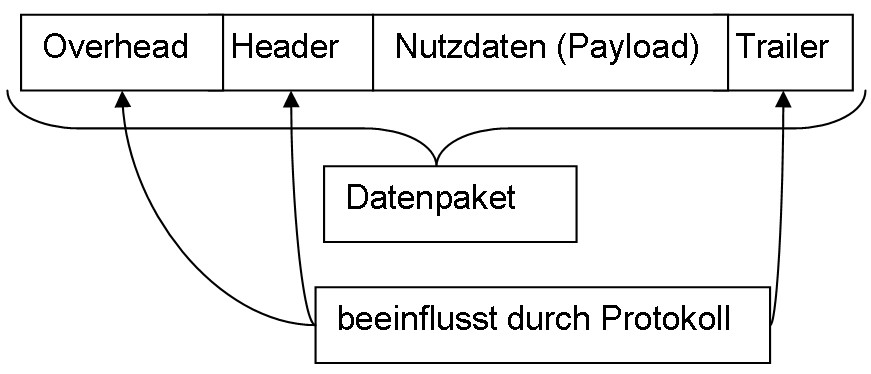
\includegraphics[width=\textwidth]{pictures/datenpaket.png}
	\caption{Aufbau eines Datenpakets \cite{Header-Dat}}
	\label{fig:datenpaket}
\end{figure}

Nachdem nun die wichtigsten Bestandteile eines Datenpakets eingeführt wurden, sind alle Grundlagen aus dem Bereich der Netzwerkarchitektur und Netzwerktechnik beschrieben, welche im Rahmen des Praktikums benötigt werden. Es wurde die Begriffe DMZ, Intranet und Internet eingeführt, sowie die wichtigsten Netzwerkprotokolle und ihr Zusammenhang zu den Datenpaketen. 

Im folgenden Kapitel wird das zugrundeliegendes Betriebssystem "Debian GNU Linux 7.11" und die Besonderheiten in der Laborumgebung in Kürze Beschrieben.
\subsection{Virtuelles Betriebsystem (Debian GNU/Linux 7.11) }\label{Linux}
Debian GNU Linux 7.11 ist ein kostenfreies und gemeinschaftliches entwickeltes Betriebssystem. Die Version 7.11, welche im Rahmen des Praktikums eingesetzt wird, gehört zu einer älteren Version und wird von Softwareentwicklern nicht mehr unterstützt. GNU Linux 7.11 unterstützt verschieden Rechnerarchitekturen wie z.B. x86(i386 \& amd64). 

Die Besonderheit im Laborpraktikum ist die, dass mit virtuellen Maschinen auf einem zugrundeliegenden Windows 10 Betriebssystems gearbeitet wird. Dies birgt einige Probleme, zum einen müssen die virtuellen Maschinen im Bereich der Netzwerkadapter einwandfrei konfiguriert sein.

Zum anderen kann mit den Maschinen nicht auf das Internet zugegriffen werden. Dies stellt ein wesentliches Problem dar, da ohne Verbindung zum Internet Paketdienste wie "Aptiude" nicht funktionieren. Aus letzterem Grund muss zwingend bei der Installation von neuen Paketen das virtuelle Image in die Maschine "eingelegt" werden. Eine andere Möglichkeit wäre, die Pakete einzelnen mit Hilfe des zugrunde liegenden Systems zu Downloaden und einzeln einzuspielen. Diese Variante stellte sich aber als sehr zeitintensiv und kompliziert heraus, da jedes Paket Abhängigkeiten mitbringt und diese zusätzlich an Versionen gebunden sind. So kann es passieren, dass dieser Prozess der Installation eine neue Problemkette im Betriebssystem schafft. Somit wurden alle Pakete, welche für die Lösung der Aufgabe benötigt wurden, mit Hilfe der bereitliegenden Linux-Images installiert.  

Eine weitere Besonderheit ist die, dass es keine grafische Benutzeroberfläche gibt, dies setzt die Arbeit "auf Konsole" voraus.  Somit muss auch mit den Linux internen Texteditoren, wie z.B. dem "VI" oder "Nano" gearbeitet werden. Dies stellt insofern ein Problem dar, da Linux in sich hochgradig "case sensitiv" reagiert. Dies bedeutet im Umkehrschluss, dass wenn ein Leerzeichen oder Komma falsch gesetzt wird, terminiert beispielweise ein Skript nicht so wie der Nutzer es vorgesehen hat. Jedoch ist es zwingend empfohlen, sämtliche Skripte auf dem virtuellen System zu schreiben, da sonst durch das Kopieren von ,beispielsweise einem Windows Betriebssystem, illegale nicht sichtbare Steuerzeichen im Skript auftreten könnten\cite{editoren-3}. 

Ein wichtiger Punkt im Zusammenspiel der Skripte und dem Betriebssystem, ist die Wahl der Shell, mit welcher es ausgeführt werden soll. Linux bietet viele verschiedene Shells an, im Rahmen des Praktikums wurde ausschließlich mit der sogenannten "bash" gearbeitet, da sie unter Linux die "Standard-Login" Shell darstellt\cite{bash-2}. In sämtlichen Skripten wurde in der ersten Zeile der sogenannten "Shebang", welcher aus "\# !" besteht, eingefügt. Gefolgt von diesem wird der Ort des Interpreter angegeben, mit welchem das Skript ausgeführt werden soll. In diesem Fall sieht diese erste Zeile eines Skripts immer aus wie folgt , "\#! /bin/bash" \cite{shebang-1}. 
//korrektur bis hier her gemacht 17:00 Uhr
Damit wurden alle wichtigen Besonderheiten des Betriebssystem im Rahmen des Praktikums eingeführt. Im nächsten Kapitel wird das "IP-Tables" Paket von Linux eingeführt, da dieses einen Grundstein für die Lösung der Aufgabenstellung im Bezug auf die internen Firewalls darstellt. 
\subsection{IP-Tables}\label{iptables}
In diesem Kapitel werden die Möglichkeiten des Linux Pakets "IP-Tables" zur Filterung von Paketen beschrieben und eingeführt. Mit Hilfe dieses Pakets werden die für die Lösung erforderlichen Firewall-Skripte erstellt.  

\subsubsection{Allgemein}
Das Paket "IP-Tables" ist standardmäßig in der Linux Installation enthalten. Es kann aber auch einfach über den Paketmanager, mit Hilfe des Befehls "apt-get install iptables" installiert werden. In diesem Fall war das Paket schon installiert und musste nicht mehr manuell installiert werden. 

Grundlegend stellt das IP-Table einen Paketfilter dar, welches Pakete auf IP-Ebene auf Basis zuvor definierter Regeln filtert. Empfangene Pakete werden überprüft, bevor sie weitergeleitet werden. Umgekehrt werden ausgehende Pakete geprüft, bevor sie den Rechner verlassen. Es kann aber auch sein, dass der Rechner als Router fungiert, so müssen alle Pakete geprüft werden, während diese weitergeleitet werden sollen. 
\subsubsection{Funktionsweise}
Die Paketprüfung wird dreistufig in einer Hierarchie durchgeführt. Die folgenden drei Stufen gibt es:
\begin{itemize}
\item Tabellen,
\item Chains (Ketten),
\item Filterregeln.
\end{itemize}

Wird eine definierte Regel in einer Chain oder Tabelle gefunden, wird die hinterlegte Aktion ausgeführt. Wenn keine Regel definiert wurde, wird eine allgemein definierte sogenannte Policy ausgeführt.

\subsubsection{Tabellen}
In einer Tabelle werden die Filterregeln zu Gruppen zusammengefasst und nach der grundlegenden Aufgabe sortiert. Insgesamt gibt es vier Tabellen, in denen eine Regel eingeordnet werden kann. In der folgenden Tabelle werden diese vier Tabellen und ihre Eigenschaften beschrieben\cite{iptables-1}. 

\begin{table}[!h]
\centering
\resizebox{\textwidth}{!}{%
\begin{tabular}{|l|l|}
\hline
\multicolumn{1}{|c|}{\textbf{Tabelle}} & \multicolumn{1}{c|}{\textbf{Beschreibung}} \\ \hline
\textbf{filter} & Standardtabelle, hier werden nur die grundlegenden Regeln hinterlegt. \\ \hline
\textbf{nat} & (Network Address Translation) Tabelle für die Adressumsetzung und für das Port-Forwarding. \\ \hline
\textbf{mangel} & Tabelle bei gewünschter Manipulation von Paketen. \\ \hline
\textbf{raw} & Tabelle für Ausnahmen beim Connection tracking. \\ \hline
\end{tabular}%
}
\caption{IP-Tables: Tabellen}
\label{Tables: Tabellen}
\end{table}
 
\subsubsection{Chains}
In jeder Tabelle sind sog. "Chains" enthalten, welche festlegen, wann ein Paket geprüft wird, bevor es, zum Beispiel, verschickt werden soll. In der folgenden Tabelle werden alle fünf verschiedenen möglichen "Chains" beschrieben\cite{iptables-1}. 

\begin{table}[!h]
\centering
\resizebox{\textwidth}{!}{%
\begin{tabular}{|l|l|l|}
\hline
\textbf{Chain} & \textbf{Tabelle} & \textbf{Beschreibung} \\ \hline
\textbf{INPUT} & filter, mangle & Relevant für alle Pakete, welche an einen lokalen Prozess gerichtet sind. \\ \hline
\textbf{OUTPUT} & filter, nat, mangle, raw & Relevant für alle Pakete, welche von einem lokalen Prozess abstammen. \\ \hline
\textbf{FORWARD} & filter, mangle & Relevant für alle Pakete, welche geroutet werden sollen. \\ \hline
\textbf{PREROUTING} & nat, mangle, raw & Relevant für alle Pakete, bevor sie geroutet werden sollen. \\ \hline
\textbf{POSTROUTING} & nat, mangle & Relevant für alle Pakete, nachdem sie geroutet wurden. \\ \hline
\end{tabular}%
}
\caption{IP-Tables: Chains}
\label{IP-Tables: Chains}
\end{table}

\subsubsection{Filterregeln}
Sobald ein Paket auf eine Filterregel trifft, muss definiert werden, wie mit dem Paket umgegangen werden soll. Dafür gibt es vier Optionen, welche am häufigsten Anwendung finden \cite{iptables-1}. Diese sind:
\begin{itemize}

\item ACCEPT: Das Paket wird akzeptiert und angenommen,
\item DROP: Das Paket wird, ohne Nachricht an den Absender, abgelehnt,
\item REJECT: Das Paket wird, mit Nachricht an den Absender, abgelehnt,
\item LOG: Die Daten des Pakets werden in den System Log geschrieben und es wird mit der nächsten Regel der Chain fortgefahren. 

\end{itemize}

Für dieses Laborpraktikum sind die beschriebenen vier Filterregeln ausreichend, im Kontext des IP-Tables Pakets bietet Debian/Linux noch weitere Optionen an. 
 
\subsubsection{Policies}

Da sich aus den beschriebenen Optionen eine große Anzahl an Möglichkeiten für Filteregeln für die einzelnen Pakete ergibt, gibt es sogenannte "Policies". Diese "Policies" setzen sich aus der Filterregel, der Chain und Aktion zusammen \cite{iptables-1}. Exemplarisch könnte ein Befehl für Input, Drop oder Forward, wie folgt aussehen: 
\begin{lstlisting}[caption={Policies},label=lst:policy]
iptables -P INPUT DROP
iptables -P OUTPUT DROP
iptables -P FORWARD DROP
\end{lstlisting}

Alle beschriebenen Möglichkeiten von IP-Tables wurden im Rahmen des Praktikums für die Lösung der Problemstellung eingesetzt. Dies ist jedoch nur ein Teil der Möglichkeiten von IP-Tables und spiegelt nicht den kompletten Funktionsumfang wieder. 
Im folgenden Kapitel wird eine Einführung in die Grundlagen einer Public Key Infrastructure gegeben, wie sie auch für das Praktikum benötigt wird.
\subsection{Public Key Infrastructure}\label{PKI}
Eine Public Key Infrastructure ist ein System, anhand dessen digitale Zertifikate ausgestellt, geprüft und verteilt werden können. Diese ausgestellten Zertifikate werden dann für die sichere Kommunikation zwischen Netzwerkteilnehmern genutzt.
\subsubsection{Aufbau einer PKI}
Eine PKI besteht grundsätzlich aus folgenden Bestandteilen

\begin{quotation}
\item [\textbf{Digitale Zertifikate:}]
Mit Hilfe der digitalen Zertifikate wird die Echtheit eines Objekts sichergestellt, zudem kann die Authentizität und Integrität mit Hilfe von kryptographischen Verfahren nachgeprüft werden. Ein Zertifikat enthält die Schlüssel, welche zur Authentifizierung und Ver- und Entschlüsselung der zu übertragenden Daten sorgen. Die Ausstellung eines digitalen Zertifikats erfolgt durch die Zertifizierungsstelle (CA)
\item [\textbf{Zertifizierungsstelle (CA):}]Eine Zertifizierungsstelle (CA), bildet den Kern einer PKI. Sie ist für das Herausgeben der Zertifikate verantwortlich und trägt die Verantwortung für die Integrität dieser. 
\item [\textbf{Registrierungsstelle (RA):}]Eine Registrierungsstelle (RA), ist eine Organisation bei der Zertifikate beantragt werden können. Dies können Personen, Maschinen oder auch untergeordnete Zertifizierungsstellen sein. Die RA prüft den Zertifizierungsantrag und nach erfolgreicher Prüfung, kann dieses dann durch die Zertifizierungsstelle signiert werden. 
\item [\textbf{Zertifikatssperrliste (CRL):}] Eine Zertifikatssperrliste(CRL), enthält alle Zertifikate, welche vor ihrem eigentlich Ablaufdatum ungültig geworden sind. Dies kann bspw. durch einen geknackten Algorithmus bei einem der Schlüssel passieren. 
\item [\textbf{Verzeichnisdienst (Directory Service):}] Ein Verzeichnisdienst, enthält alle ausgestellten Zertifikate. In Unternehmen ist dieser Dienst meistens durch einen LDAP-Server realisiert. 
\item [\textbf{Validierungsdienst (VA)}:] Ein Validierungsdienst(VA), stell die Möglichkeit bereit ein Zertifikat in Echtzeit zu prüfen. Im Normalfall ist dies durch OCSP oder SCVP realisiert.  
\end{quotation}

Im Rahmen des Praktikums wurde eine solche PKI bereits zur Verfügung gestellt. Im nächsten Abschnitt wird die Erstellung eines Server-Zertifikats gezeigt, wie es auch für die Lösung der Aufgabenstellung erforderlich ist. 
\subsubsection{Erstellung eines Server-Zertifikats}
Der Ablauf für die Erstellung eines Server-Zertifikats besteht aus insgesamt sechs Schritten, diese werden nun ihrer Reihenfolge nach beschrieben. 

\begin{enumerate}
\item Der Benutzer muss sich zuerst ein Schlusslpaar erzeugen (privater/öffentlicher)\cite{JueNeuSaDue}.
\item Auf der CA-Seite, kann sich der der Benutzer nun die req.cnf runterladen. In dieser Datei sind alle Grundeinstellungen der CA enthalten\cite{JueNeuSaDue}. 
\item Aus der req-Datei und dem Schlüssel kann der Benutzer nun einen Zertifikats-Request erstellen (Request, Fileextension csr). Dieser Request enthält den öffentlichen Schlüssel, welcher dann von der CA beglaubigt wird\cite{JueNeuSaDue}. 
\item Jetzt kann die csr-Datei auf die CA-Seite hochgeladen werden\cite{JueNeuSaDue}. 
\item Der Request wird nun auf dem CA-Server verarbeitet und das signierte Zertifikat für den Benutzer auf der Seite der CA zum Download bereitgestellt\cite{JueNeuSaDue}. 
\item Diese crt-Datei, welche nun heruntergeladen werden kann, kann nun einfach für die Sicherung der Netzwerkkomponenten genutzt werden, bspw. für den VPN-Client oder VPN-Server\cite{JueNeuSaDue}.  
\end{enumerate}

Für die Lösung der Aufgabenstellung muss dieser Vorgang insgesamt zwei Mal durchgeführt werden, da für Client und Server ein solches Server-Zertifikat benötigt wird. Zu beachten ist auch, dass die Software OpenSSL zwingend für die Erstellung des privaten Schlüssels, installiert sein muss.

Der Gesamtprozess zur Erstellung eines Server-Zertifikats wird in Abbildung \ref{fig:Zertifikaserstellung} nochmals verdeutlicht.  
\begin{figure}[!h]
	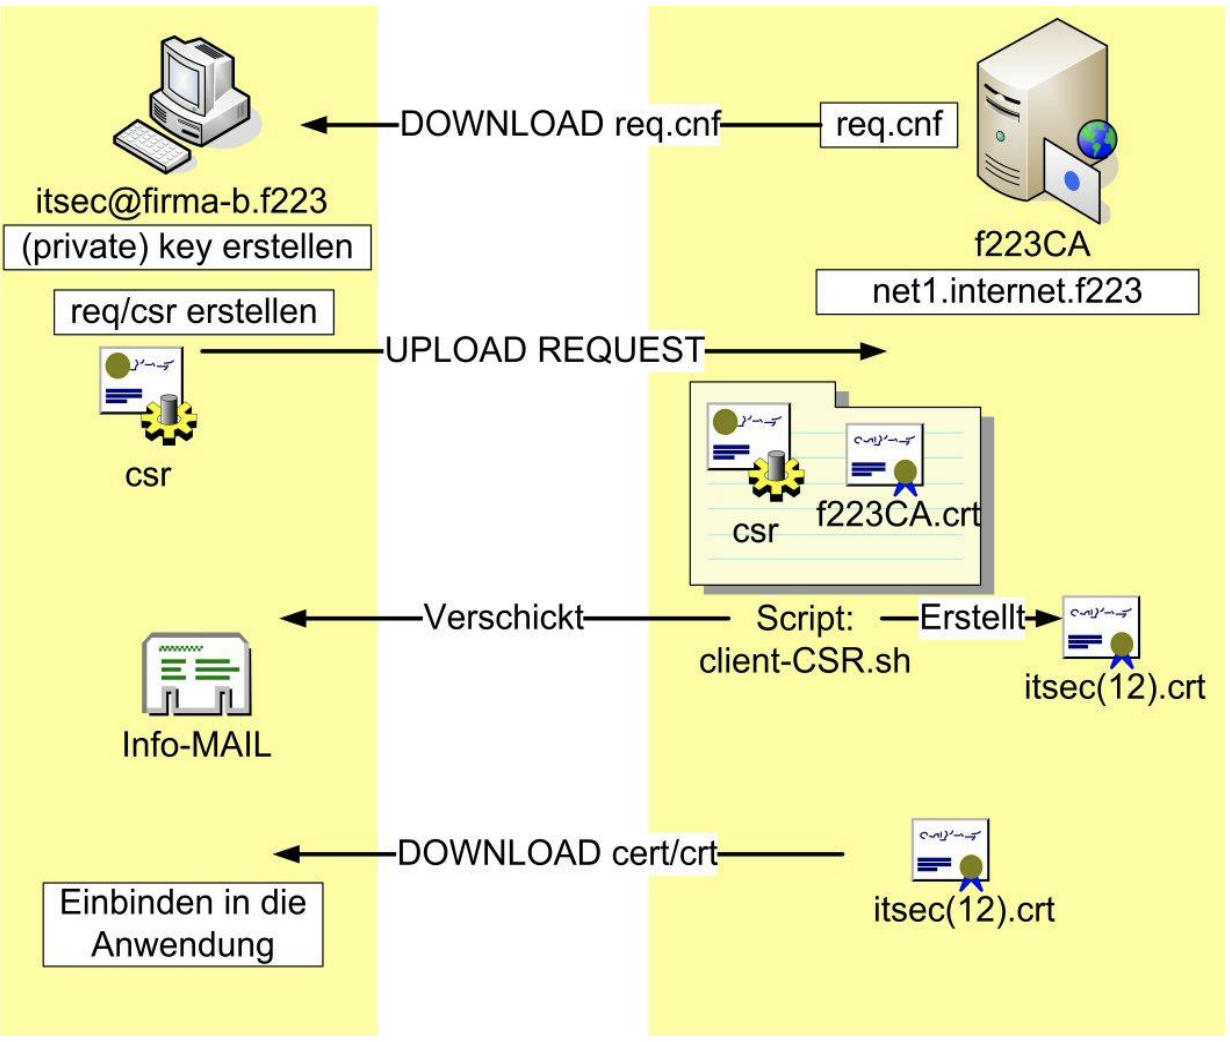
\includegraphics[width=\textwidth]{pictures/Zertifikatserstellung.png}
	\caption{Zertifikatserstellung im Labor\cite{JueNeuSaDue}}
	\label{fig:Zertifikaserstellung}
\end{figure}
\newpage
Im folgenden Abschnitt wird, die für die Umsetzung der VPN-Verbindung benötigte Software OpenVPN eingeführt. 
\newpage
\subsection{OpenVPN}\label{openvpn}

Für die Lösung der Problemstellung wurde die Software OpenVPN genutzt, da sie den Anforderungen an die Aufgabenstellung entspricht. Da OpenVPN zwingend die Software OpenSSL voraussetzt und diese ohnehin für die Erstellung der privaten Schlüssel genutzt wird, war die Wahl schnell getroffen\cite{openV-1}. 

\subsubsection{Grundlagen}
OpenVPN ist eine frei verfügbare Software für die Einrichtung eines virtuellen Netzwerks, über eine verschlüsselte TLS/SSL-Verbindungen. Wie bereits angesprochen, erfolgt die Verschlüsselung mit Hilfe von OpenSSL. Es kann wahlweise UPD oder TCP als Transportprotokoll eingesetzt werden. Zur Authentifizierung bietet OpenVPN das sogenannte Pre-shared Key Verfahren oder eine Authentifizierung über Zertifikate, welches im Rahmen des Praktikums auch eingesetzt wurde\cite{openV-1}. 

OpenVPN bietet grundlegend folgende Eigenschaften:

\begin{itemize}
\item Verfügbarkeit verschiedenen Betriebsmodi (Bridging oder Routing),
\item Tunnelung in beliebige Subnetze 
\item Verschiedene Verschlüsselungsarten (Pre-shared Key / Zertifikate)
\item Skalierbarkeit bei VPN-Serverfarmen
\end{itemize}

\subsubsection{Authentifizierung}
Wie schon angesprochen, verfügt OpenVPN über zwei verschiedene Methoden zur Authentifizierung, folgend werden beide gegenüberstellt. 

\begin{quotation}
\item[\textbf{Pre-shared Key:}]
ist ein symmetrisches Verfahren, der Schlüssel wird im VPN-Server erstellt und an die Clients verteilt. Es handelt sich um ein sehr einfaches Verfahren. Jedoch ist es nicht sehr sicher, da es nur einen Schlüssel gibt und falls dieser korrumpiert werden sollte, müssten sämtliche Kommunikationsteilnehmer neue Schlüssel erhalten und wären potentiell in Gefahr\cite{openV-1}. 

\item[\textbf{Zertifikatsbasiert:}]
ist ein auf dem TLS-Protokoll basierendes Verfahren, welches aktuell als sehr sicher klassifiziert wird. Dieses Verfahren beruht auf privaten und öffentlichen Schlüsselpaaren. Der Server und der Client erhalten jeweils ein öffentliches und privates Zertifikat. Mit Hilfe von easy-rsa könnten auch sehr einfach die benötigen Zertifikate erstellt werden. Diese Aufgabe wird jedoch im Praktikum durch die PKI übernommen. Allgemein ist dieses Verfahren sicherer als das Pre-shard Key, es bringt aber auch eine höhere Komplexität bei der Umsetzung mit sich\cite{openV-1}. 
\end{quotation} 

\subsubsection{Kommunikation}

Mittels OpenVPN kann entweder eine Client-Server Verbindung aufgebaut werden, auch Roadwarrior genannt, oder, wie in der Aufgabenstellung gefordert, eine Site-to-Site Verbindung. Im Standard wird die Kommunikation über das zustandslose UDP-Protokoll abgewickelt. Diese kann jedoch auch auf das TCP-Protokoll umgestellt werden\cite{openV-1}. 

Zudem bietet OpenVPN auch verschiedene Netzwerkmodi an Bridging-Mode (Tap-Device) und Routing-Mode (Tun-Device). 
Diese zwei Modi werden folgend gegenübergestellt. 

\begin{quotation}
\item[\textbf{Bridging-Mode(Tap-Device):}]
in diesem Modus wird ein vollständiges Tunneln des Ethernet-Frames (Layer 2) vorgenommen. Der Client erhält in diesem Fall die IP-Adresse des aktuellen Subnetzes. Die Broadcast müssen in dem Fall auch weitergeleitet werden, um eine potentielle Namensauflösung via SMB-Protokoll zu gewährleisten\cite{openV-1}.

\item[\textbf{Routing-Mode (Tun-Device):}]
in diesem Modus werden ausschließlich IP-Pakete (Layer 3) über einen verschlüsselten Tunnel verschickt. Jeder Kommunikationspartner bekommt eine virtuelle IP-Adresse eines fiktiven Subnetzes. Somit ist der Zugriff auf das dahinter liegenden Netz standardmäßig nicht möglich. Dies muss dann über die Routing-Tabellen der Firewalls  oder IP-Forwarding realisiert werden\cite{openV-1}.
\end{quotation}

In der folgenden Tabelle \ref{my-Tun/Tap} werden abschließend für dieses Kapitel noch die Vor- und Nachteile der beiden beschriebenen Modi gegenüber gestellt. 
\newpage
\begin{table}[!h]
\centering
\resizebox{\textwidth}{!}{%
\begin{tabular}{|l|l|l|}
\hline
 & \textbf{Bridging-Modus (Tap-Device)} & \textbf{Routing-Modus(Tun-Device)} \\ \hline
\textbf{Vorteile} & \begin{tabular}[c]{@{}l@{}}Agiert wie ein eigenständiger Netzwerkadapter\\ \\ Verschiedene Netzwerkprotkolle verfügbar\\ \\ Client ist transparent im Zielnetz\end{tabular} & \begin{tabular}[c]{@{}l@{}}Geringer Traffic-Overhead\\ \\ Da kein Ehternet-Layer, geringe Bandbreite\\ \\ Gute Skalierbarkeit\end{tabular} \\ \hline
\textbf{Nachteile} & \begin{tabular}[c]{@{}l@{}}Schlechte Skalierbakeit\\ \\ Hoher Broadcast-Overhead am VPN-Tunnel\end{tabular} & \begin{tabular}[c]{@{}l@{}}Nur IP-Pakete möglich \\ \\ Keine Broadcasts möglich\end{tabular} \\ \hline
\end{tabular}%
}
\caption{Bridging-Mode vs. Routing-Mode}
\label{my-Tun/Tap}
\end{table}

Für die Lösung der Aufgabe wurde der Routing-Mode (Tun-Device) eingesetzt. 

Mit Abschluss dieses Kapitel wurden alle theoretischen Grundlagen, welche für den Rahmen des Laborpraktikums relevant sind, eingeführt. Im anschließenden Kapitel wird die Lösungsskizze für die Problemstellung beschrieben. 
 
% !TEX encoding = UTF-8 Unicode
\section{Lösungsskizze}\label{loesungsskizze}
In diesem Kapitel wird sich mit dem Thema befasst, wie sich eine Site-to-Site VPN Verbindung, die die Firmen A und B wie in Kapitel \ref{laborumgebung} beschrieben, verbindet.
Dazu waren zu Beginn mehrere Vorüberlegungen zu tätigen. Dies sind zum einen: wie wird das innere Netz der Firmen A und B geschützt und zum anderen, welcher VPN Dienst für diesen Zweck verwendet werden kann und welche weiteren Strategien bei der Umsetzung der Security Policies der Firmen benötigt werden. 
\subsection{Firewall}\label{firewallloesung}
Wenn eine Firewall aufgebaut werden soll, muss zu Beginn überlegt werden, welche allgemeine Strategie mit der Firewall gefahren werden soll. Das heißt, sollen alle Verbindungen standardmäßig freigegeben werden und nur explizit nicht erlaubte Verbindungen geblockt werden (Default-Allow-Strategy), oder sollen alle Verbindungen blockiert werden und nur die die explizit erlaubt wurden, geöffnet werden (Default-Deny-Strategy). 

Im Standardfall wird in Unternehmen die Strategie Default-Deny verwendet, weshalb auch im Versuchsaufbau diese Strategie gewählt wurde. Eine Firewall wird mit Hilfe des Userspace-Programmes IPTABLES (siehe Kapitel \ref{iptables}) unter Linux realisiert. Dafür wird eine Rules Datei (nachfolgend Skript genannt) angelegt.Iin dieser werden die Einstellungen und Regeln für die Firewall definiert. Zu Beginn des Skriptes wird der Interpreter für den Code angegeben. Dann wird begonnen, die durch die Default Strategie vorgegebenen Default Policies umzusetzen (siehe Auflistung \ref{lst:defaultPolicy}). Dabei sagt das -P, dass die Policy angesprochen werden soll, das INPUT, OUTPUT und FORWARD bezieht sich auf die im Kapitel \ref{iptables} vorgestellten Chains. DROP sagt dabei aus, dass die eintreffenden Pakete, wenn keine weiteren Regeln definiert oder zutreffen nicht weitergeleitet und "fallengelassen'' werden sollen.
\newline
\lstset{
	basicstyle=\footnotesize, frame=tb,
	xleftmargin=.2\textwidth, xrightmargin=.2\textwidth
}
\begin{lstlisting}[caption={Default Policy IPTABLE},label=lst:defaultPolicy]
#Verwenden der Tabelle FILTER
*filter
-P INPUT DROP
-P OUTPUT DROP
-P FORWARD DROP
\end{lstlisting}
\vspace{\baselineskip}
Nach dem die Default Policy erfolgreich eingeführt wurde, werden die feingranularen Regeln definiert. Dies setzt die Verwendung des Befehles -F voraus. Dieser löscht alle bisherigen Filterregeln, um die nachfolgenden neu definierten Regeln einzuführen. Bei Linux ist dabei zu beachten, dass ein Teil der Interprozesskommunikation über das interne Netzwerk läuft. Dafür ist es nötig diese Kommunikation zuzulassen. 
Dies geschieht analog, wie in der nachfolgenden Auflistung \ref{lst:interprozess} zu sehen ist. 
\newline
\lstset{
	basicstyle=\footnotesize, frame=tb,
	xleftmargin=.2\textwidth, xrightmargin=.2\textwidth
}
\begin{lstlisting}[caption={Interprozesskommunikation zulassen},label=lst:interprozess]
# Interprozesskommunikation Verbindungen erlauben
-A INPUT -i lo -j ACCEPT
-A OUTPUT -o lo -j ACCEPT
\end{lstlisting}
\vspace{\baselineskip}
Dabei sagt das ''-A'' aus, an welche Chain diese Regel angehängt werden soll. Das ''-i'' ist dabei die Option, über welches Netzwerkinterface das Paket eingegangen ist, beziehungsweise ''-o'', über welches das Paket versendet werden soll. In diesem Fall das ``lo'' Netzwerkinterface. Wenn alle Prüfregeln auf das Paket zutreffen, wird mit ''-j'' entschieden, wie mit dem Paket verfahren werden soll, in diesem Beispiel soll es mit ACCEPT akzeptiert werden. 
\newline
\lstset{
	basicstyle=\footnotesize, frame=tb,
	xleftmargin=.2\textwidth, xrightmargin=.2\textwidth
}
\begin{lstlisting}[caption={Weitere allgemeine Firewallregeln},label=lst:allgemeineRegeln]
# Erlaube ICMP Befehle
-A INPUT -p icmp -j ACCEPT
-A OUTPUT -p icmp -j ACCEPT

# Erlaube SSH Verbindung
-A INPUT -p tcp --dport 22 -j ACCEPT

# Alle Verbindungen von innen nach aussen zulassen
-A FORWARD -i eth0 -o eth1 -m state --state NEW -j ACCEPT

# Erlaube nur bereits aufgebaute 
# Verbindungen von aussen nach innen
-A FORWARD -m state --state RELATED,ESTABLISHED -j ACCEPT
\end{lstlisting}
\vspace{\baselineskip}
Die, in der Auflistung \ref{lst:allgemeineRegeln} dargestellten Regeln, sind allgemeine Regeln für die Firewall. Diese erlauben das Empfangen von Pinganfragen, den Fernzugriff mittels SSH, alle neuen Verbindungen von innen nach außen und alle bereits aufgebauten Verbindungen, beziehungsweise alle Verbindungen, die einen Bezug auf eine andere Verbindung besitzen. In der nachfolgenden Tabelle \ref*{tab:iptablesOptionen} werden die hier verwendeten Optionen nochmals näher beschrieben.
\begin{table}[h]
	\centering
\begin{tabular}{|p{2cm}|p{13cm}|}
	\hline 
	Optionen & Beschreibung \\ 
	\hline 
	-p & Gibt das Protokoll an welches verwendet werden soll hier icmp(Ping), tcp \\ 
	\hline 
	-dport & Gibt den Destinationport an, auf den zugegriffen werden soll hier 22 \\ 
	\hline
	eth0,eth1 & bezieht sich auf das verwendete Netzwerkinterface \\ 
	\hline 
	-m state & die entreffenden Pakete sollen auf den Status überprüft werden \\ 
	\hline 
	--state & Status der eintreffenden Pakete, hier NEW, RELATED,ESTABLISHED \\ 
	\hline 
\end{tabular} 
\caption{IPTABLES Optionen und Beschreibung} \label{tab:iptablesOptionen}
\end{table}
Nach den allgemeine Regeln müssen nun die VPN spezifischen Regeln definiert werden. Dazu muss man die auf den VPN Ports eintreffenden und ausgehenden Pakete betrachten. Diese Ports sind entweder 1194 oder 1195. In der Auflistung \ref{lst:VPNRegeln} sind VPN Regeln zusehen. Eine Besonderheit bei VPN ist, das zum einen alle Verbindungen, die über das Netzwerkinterface tun0 eintreffenden Pakete ohne Überprüfung an das Inteface eth0 übergeben werden. Des weiteren wird noch die Tabelle NAT benötigt, was das ''*nat'' angibt. In dieser Tabelle gibt es die Chain POSTROUTING. Über diese kann nachträglich der Verkehrsheader eines Paketes verändert werden. MASQUERADE hat dabei die Funktion, dass wenn ein Paket versendet wird, die Source-IP-Adresse so verändert wird, dass nur noch die IP-Adresse des Firewallservers ersichtlich ist. Dies hat den Grund, dass von außen nicht ersichtlich wird, welche IP-Adressen sich hinter der Firewall befinden und es so Angreifern erschwert wird, diese anzugreifen.
\newline
\lstset{
	basicstyle=\footnotesize, frame=tb,
	xleftmargin=.01\textwidth, xrightmargin=.01\textwidth
}
\begin{lstlisting}[caption={Weitere VPN Firewallregeln},label=lst:VPNRegeln]
# Erlaube alle Verbindungen auf den VPN Ports
-A INPUT -i eth1 -p udp --dport 1194 -m state --state NEW -j ACCEPT
-A INPUT -i eth1 -p udp --dport 1195 -m state --state NEW -j ACCEPT
-A INPUT -m state --state RELATED,ESTABLISHED -j ACCEPT
-A OUTPUT -m state --state RELATED,ESTABLISHED -j ACCEPT
-A INPUT -i tun0 -j ACCEPT

#Forwarding fuer die VPN Verbindungen
-A FORWARD -i tun0 -o eth0 -m state --state NEW -j ACCEPT
-A FORWARD -i eth0 -o tun0 -m state --state NEW -j ACCEPT
-A FORWARD -i tun0 -o eth0 -m state --state RELATED,ESTABLISHED -j ACCEPT
-A FORWARD -i eth0 -o tun0 -m state --state RELATED,ESTABLISHED -j ACCEPT
COMMIT

#Verwenden der Tabelle NAT
*nat

#Loeschen der vorhandenen Regeln
-F

-A POSTROUTING -o eth1 -j MASQUERADE
COMMIT
\end{lstlisting}
\vspace{\baselineskip}
Nach dem Erstellen des Skriptes, muss dieses nun eingespielt werden. Dazu wird der Befehl ''iptables-restore'' verwendet. Dieser wird exemplarisch in der Auflistung \ref{lst:fwrestorea} veranschaulicht, dabei liegt das Skript im Ordner ''etc''.
\newline
\lstset{
	basicstyle=\footnotesize, frame=tb,
	xleftmargin=.2\textwidth, xrightmargin=.2\textwidth
}
\begin{lstlisting}[caption={Einspielen des Firewallskriptes der Firma a},label=lst:fwrestorea]
iptable-restore < etc/iptables.firewall-a.rules
\end{lstlisting}
\vspace{\baselineskip}
Nach dem das Skript eingespielt wurde, muss dieses noch so konfiguriert werden, sodass es nach einem Serverneustart automatisch neu eingespielt wird. Dazu könne zwei Arten verwendet werden. Zum einen mit Hilfe des ''if-pre-up.d'' Directories. Dabei wird eine neue Datei angelegt mit dem Namen ''iptables''. In der Auflistung \ref{lst:neustart} wird der Inhalt, der neu angelegten Datei gezeigt. Nun muss die Datei noch ausführbar gemacht werden, dies geschieht mit Hilfe des Befehls ''chmod +x''
\newline
\lstset{
	basicstyle=\footnotesize, frame=tb,
	xleftmargin=.2\textwidth, xrightmargin=.2\textwidth
}
\begin{lstlisting}[caption={Automatisches Laden des Iptablesskriptes bei Serverneustart},label=lst:neustart]
#!/bin/bash
/sbin/iptasbles-restore < /etc/iptables.fwirewall-a.rules
\end{lstlisting}
\vspace{\baselineskip}
Die zweite Möglichkeit des automatischen Neuladens der Firewall, ist mit Hilfe des Tools ''iptables-peristent''. Dieses Tool muss mit ''aptitute'' installiert werden. Nach dem das Tool installiert wurde, können mit dem Befehl ''iptables-save > /etc/iptables/rules.v4'' die Regeln für jeden Neustart automatisch geladen werden. 
\newline 
Eine weitere Konfiguration die vorgenommen werden muss, ist das Akzeptieren des Forwardings. Dazu muss im Verzeichnis ''/proc'' die Datei ''/proc/sys/net/ipv4/ip\_forward'' die Zeile in der Auflistung \ref{lst:forward} eingefügt werden. Zu Beginn steht in dieser Datei lediglich eine ''0'' diese muss ersetzt werden durch eine ''1'' dies aktiviert das Forwarding.\newline
\lstset{
	basicstyle=\footnotesize, frame=tb,
	xleftmargin=.2\textwidth, xrightmargin=.2\textwidth
}
\begin{lstlisting}[caption={Forwarding aktivieren},label=lst:forward]
/bin/echo "1" > /proc/sys/net/ipv4/ip_forward
\end{lstlisting}
\vspace{\baselineskip}
Wurden all diese Einstellungen vorgenommen, kann  mit der Konfiguration der Site-toSite VPN Verbindung begonnen werden, was im nachfolgenden Kapitel beschrieben wird.



\subsection{VPN}
Nach dem die Firewall auf den Servern der Firma A und B eingerichtet wurde, muss nun die VPN Verbindung erstellt werden. Dazu dient der Firewallserver der Firma A als Server und der Firewallserver der Firma B als Client. Diese Einrichtung wird in diesem Kapitel näher beschrieben. \newline
Dafür muss zu Beginn auf beiden Servern das in Kapitel \ref{openvpn} vorgestellte Tool OpenVPN installiert werden. Dies geschieht, wie schon im Kapitel \ref{firewallloesung}  erwähnt, mit dem Tool ''aptitute''. Nach der Installation müssen, wie nachfolgend erklärt, für den Server der Firma A und B ein Serverzertifikat erstellt werden.

\subsubsection{Serverzertifikate}
Wie schon in Kapitel \ref{PKI} erklärt, wird für die  Einrichtung eines VPN's Zertifikate benötigt. Diese werden verwendet, um eine Verbindungsverschlüsselung zu realisieren. In diesem Kapitelteil wird anhand der Firma A erklärt, wie ein solches Zertifikat in der Laborumgebung erstellt wird. Um ein Zertifikat für Firma B zu erstellen, ist der gleiche Prozess notwendig. \newline
Für das Erstellen eines Zertifikates ist das Tool OpenSSL notwendig. Über OpenSSL wird ein öffentlicher und privater Schlüssel erzeugt. Nach dem diese erstellt wurden, muss von der Zertifizierungsstelle die Konfigurationsdatei geladen werden. Mit Hilfe dieser Konfigurationsdatei des privaten Schlüssels und des Tools OpenSSL wird nun eine CSR (Certificate Signing Request) Datei erzeugt. Nach dem diese Datei erzeugt wurde, muss diese zur Zertifizierungsstelle hochgeladen werden. Nach dem Upload der Datei (Zertifikat), muss diese nun signiert werden. Dies wird im Labor mit einem Shellskript realisiert. Nach dem Signieren kann nun das fertige Zertifikat geladen und auf dem Server 
abgelegt werden. In der Auflistung \ref{lst:openssl}  werden die einzelnen Befehle zur Erstellung der Schlüssel und der CSR Datei gezeigt und die einzelnen Befehle in der Tabelle \ref{tab:openSSLOptionen} näher beschrieben.\newline
\lstset{
	basicstyle=\footnotesize, frame=tb,
	xleftmargin=.2\textwidth, xrightmargin=.2\textwidth
}
\begin{lstlisting}[caption={Erzeugen eines privaten Schlüssels mit OpenSSL},label=lst:openssl]
#Privaten Schluessel erzeugen
openssl genrsa -out firma-A.key 2048

#Request erstellen - CSR-Datei
openssl req -new -key firma-A.key -config req.cnf -reqexts v3_req_srv -out CSR-firma-A.csr
\end{lstlisting}
\vspace{\baselineskip}
\begin{table}[h]
	\centering
\begin{tabular}{|l|l|}
	\hline 
	Befehle & Beschreibung \\ 
	\hline 
	openssl & Tool zur Erstellung von privaten Schlüsseln \\ 
	\hline 
	genrsa & Befehl zum erstellen des Schlüssels mittels RSA \\ 
	\hline 
	-out & Ausgabe des Schlüssels in angegebene Datei \\ 
	\hline 
	firma-A.key & Name der Schlüsseldatei \\ 
	\hline 
	2048 & Schlüssellänge in Bits \\ 
	\hline 
	req -new & Erzeugen eines neuen Requests \\ 
	\hline 
	-config & laden der Konfigurationsdatei req.cnf \\ 
	\hline 
	-reqexts & Erweiterung des X.509 Formates \\ 
	\hline 
\end{tabular} 
\caption{Befehle zur Erstellung eines Privaten Schlüssels mittels OpenSSL} \label{tab:openSSLOptionen}
\end{table}

\subsubsection{Server Firma A}
Nach dem die Zertifikate, wie im vorherigen Kapitel erstellt wurden, kann nun mit dem Konfigurieren des VPN-Servers begonnen werden. Dazu wird zuerst mittels Root-Users das Verzeichnis ''/etc/opnevpn'' erstellt. Nach dem dieses erstellt wurde, werden zwei Unterverzeichnisse ''/etc/openvpn/certs'' und ''/etc/openvpn/keys'' angelegt. In das Unterverzeichnis ''certs'' werden das Serverzertifikat ''fw2-firma-A.crt'' und die Zertifikatschain (von der Zertifizierungstelle) kopiert. In das Unterverzeichnis ''keys'' wird der private Schlüssel verschoben. Da der private Schlüssel geheimgehalten werden soll, muss die Berechtigung für das Unterverzeichnis noch geändert werden. Dies wird mit dem Befehl ''chmod -R 600 /etc/openvpn/keys/'' bewerkstelligt. Der nächste Schritt ist das erstellen des Diffie-Hellman Schlüssels. Dieser Schlüssel wird später benötigt um später die Verbindung symmetrisch zu verschlüsseln. Der dafür notwendige Befehl wird in der Auflistung \ref{lst:DH} gezeigt.\newline
\lstset{
	basicstyle=\footnotesize, frame=tb,
	xleftmargin=.2\textwidth, xrightmargin=.2\textwidth
}
\begin{lstlisting}[caption={Erzeugen des Diffie-Hellman Schlüssels},label=lst:DH]
openssl dhparam -out dh2048.pem 2048
\end{lstlisting}
\vspace{\baselineskip}
Eine besondere Eigenschaft des Site-to-Site VPN's ist, dass man für jeden einzelnen Clienten eine besondere Konfiguration ''pushen'' kann. Dies bringt den Vorteil, dass, wie hier verwendet, ein Client die Infrastruktur hinter der Firewall so verwenden kann, als wäre sie ein Teil seiner eigenen Infrastruktur. Dazu muss ein weiteres Unterverzeichnis mit dem Namen ''client\_configs" erstellt werden. Darin muss eine Datei angelegt werden, das den gleichen Namen trägt wie das Clientzertifikat. In dieser Datei werden die Konfigurationsdaten für den Clienten geschrieben, wie in Auflistung \ref{lst:clientconf} zu sehen ist.\newline
\lstset{
	basicstyle=\footnotesize, frame=tb,
	xleftmargin=.2\textwidth, xrightmargin=.2\textwidth
}
\begin{lstlisting}[caption={Clientkonfigurationsdatei fw-firma-b},label=lst:clientconf]
iroute 192.168.70.0 255.255.255.0
iroute 192.168.80.0 255.255.255.0
\end{lstlisting}
\vspace{\baselineskip}
Das ''iroute'' Statement gibt dem Client an, welche IP-Adressen von ihm angesprochen werden können. \newline Nun muss als letztes die OpenVPN Konfigurationsdatei erstellt und angepasst werden. Dazu können die bei der Installation von OpenVPN mitgelieferten Beispieldateien verwendet werden und nach und nach an den Verwendungszweck angepasst werden. Für die Konfiguration für den Server wird die ''server.conf'' benötigt.\newline
\lstset{
	basicstyle=\footnotesize, frame=tb,
	xleftmargin=.2\textwidth, xrightmargin=.2\textwidth
}
\begin{lstlisting}[caption={server.conf Datei der Firma A},label=lst:serverconf]
script-security 3

port 1194

proto udp

dev tun

tls-server
auth SHA1

ca /etc/openvpn/cert/f223CA.chain.crt
cert /etc/openvpn/cert/fw-firma-a.crt
# This file should be kept secret
key /etc/openvpn/keys/firma-A.key  

dh /etc/openvpn/dh2048.pem

server 192.168.100.0 255.255.255.0

ifconfig-pool-persist ipp.txt

route 192.168.70.0 255.255.255.0
route 192.168.80.0 255.255.255.0
push "route 192.168.30.0 255.255.255.0"
push "route 192.168.40.0 255.255.255.0"

client-config-dir /etc/openvpn/client_configs

keepalive 10 120

cipher aes-256-cbc

comp-lzo

user nobody	
group nogroup

persist-key
persist-tun

verb 3

\end{lstlisting}
\vspace{\baselineskip}
Die Auflistung \ref{lst:serverconf} zeigt die ''server.conf'' der Firma A. Dabei wird von oben nach unten die folgenden Konfigurationsbefehle abgearbeitet.
\begin{description}
	\item[script-security 3]
	Beschreibt die Skript Sicherheit, das heißt hier wird definiert wie OpenVPN externe Programme und Skripte verwenden darf. Die drei  erlaubt die Übergabe von Passwörtern an Skripte über Umgebungsvariablen.
	\item[port 1194] Definiert den Port über den der VPN Verkehr abläuft. Alternativport 1195
	\item[proto udp] Definiert über welches Protokoll kommuniziert wird. 
	\item[dev tun] Erzeugt einen gerouteten IP-Tunnel.
	\item[tls-server auth SHA1] Authentifikationskonfiguration
	\item[ca] Pfadangabe zur Zertifkatschain
	\item[cert] Pfadangabe zum Serverzertifikat 
	\item[key] Pfadangabe zum Privaten Schlüssel
	\item[dh] Pfadangabe zum Diffi-Hellman Key 
	\item[server] Spezifiziert den Server als Server und gibt den IP-Adressen den Raum des VPN Netzes an.	
	\item[ifconfig-pool-persist] Datei in dem IP-Adressen der Clients gespeichert werden, um beim nächsten Verbinden von des selben Client, diesem die gleiche IP-Adresse zu geben. 
	\item[route] Definiert die hinter dem Client liegenden IP-Adressen auf die von Serverseite aus zugegriffen werden kann.
	\item[push] IP-Adressraum der an den Client ''gepusht'' werden, die der Client annehmen darf. 
	\item[client-config-dir] Pfadangabe zur Clientkonfiguration
	\item[keepalive] Gibt an, dass nach 10 Sekunden Inaktivität ein Ping an den Client gesendet wird, nach 120 Sekunden Inaktivität wird ein weiterer Versuch unternommen sich mit dem Client zu verbinden.
	\item[cipher] Kryptographische Chiffre, über die die Verbindung zwischen Client und Server verschlüsselt wird. Dies muss beim Client der gleiche Chiffre sein.
	\item[comp-lzo] Aktiviert die Kompression der Verbindung, dies muss auch beim Client aktiviert sein.
	\item[user] Nach der Initialisierung werden die Rechte des OpenVPN Nutzers auf nobody gesetzt, da zum Starten eines VPN's Rootrechte benötigt werden. Dies ist aber während der Sitzung nicht gewollt.
	\item[group]Nach der Initialisierung werden die Rechte des OpenVPN Nutzers auf nogroup gesetzt, da zum Starten eines VPN's Rootrechte benötigt werden und dies aber während der Sitzung nicht gewollt ist.
	\item[persist-key] Sichert vor einem Keepalive Neustart die Schlüssel, um diese nicht nochmals erzeugen zu müssen.
	\item[persist-tun] Ähnlich wie persist-key, nur für das tun-interface.  
	\item[verb 3] Logging Optionen, über diese Einstellung kann die Genauigkeit des Loggens eingestellt werden.
\end{description}

\subsubsection{Client Firma B}
Ähnlich wie beim Server der Firma A, wie im Kapitel-teil zuvor, wird der Client der Firma B eingerichtet. Allerdings wird hier die ''client.conf'' benötigt und es wird kein ''client\_conf'' Verzeichnis benötigt. Nachfolgend wird in der Auflistung  die Konfigurationsdatei gezeigt und die einzelnen Begriffe nochmals erklärt.\newline
\lstset{
	basicstyle=\footnotesize, frame=tb,
	xleftmargin=.2\textwidth, xrightmargin=.2\textwidth
}
\begin{lstlisting}[caption={client.conf Datei der Firma B},label=lst:clientconf]
port 1194

client

dev tun

proto udp

remote 10.1.0.131 1194

user nobody
group nogroup

persist-key
persist-tun

ca /etc/openvpn/f223CA.chain.crt
cert /etc/openvpn/fw2.firma-b.f223.crt
key /etc/openvpn/vpnb.key

pull
auth SHA1

cipher aes-256-cbc

comp-lzo

verb 3
\end{lstlisting}
\vspace{\baselineskip}
\begin{description}
	\item[client] Spezifiziert den Client als Client
	\item[remote] Gibt die IP-Adresse und den Port des VPN-Servers an, mit dem sich der Client verbinden soll.
	\item[tls-client] Spezifiziert den Client als tls-Client
	\item[pull] holt sich über diesen Befehl die von Server ''gepushten'' Konfigurationen
\end{description}









\label{Lösungsskizze}
% !TEX encoding = UTF-8 Unicode
\section{Auswertung}
In diesem Kapitel werden die im Kapitel \ref{loesungsskizze} vorgestellten Konfigurationen verwendet und eine Auswertung der VPN Verbindung von Firma B(Client) zur Firma A(Server) gemacht.\newline
Um die VPN Verbindung zu starten wird zuerst der Server mit Hilfe des Befehls ''openvpn /etc/openvpn/server.conf'' gestartet. Nach dem der Server gestartet wurde, wird bei Firma B der Client mit ''openvpn /etc/openvpn/client.conf'' gestartet. Dabei initiiert der Client den Verbindungsaufbau. 
\begin{figure}[h]
	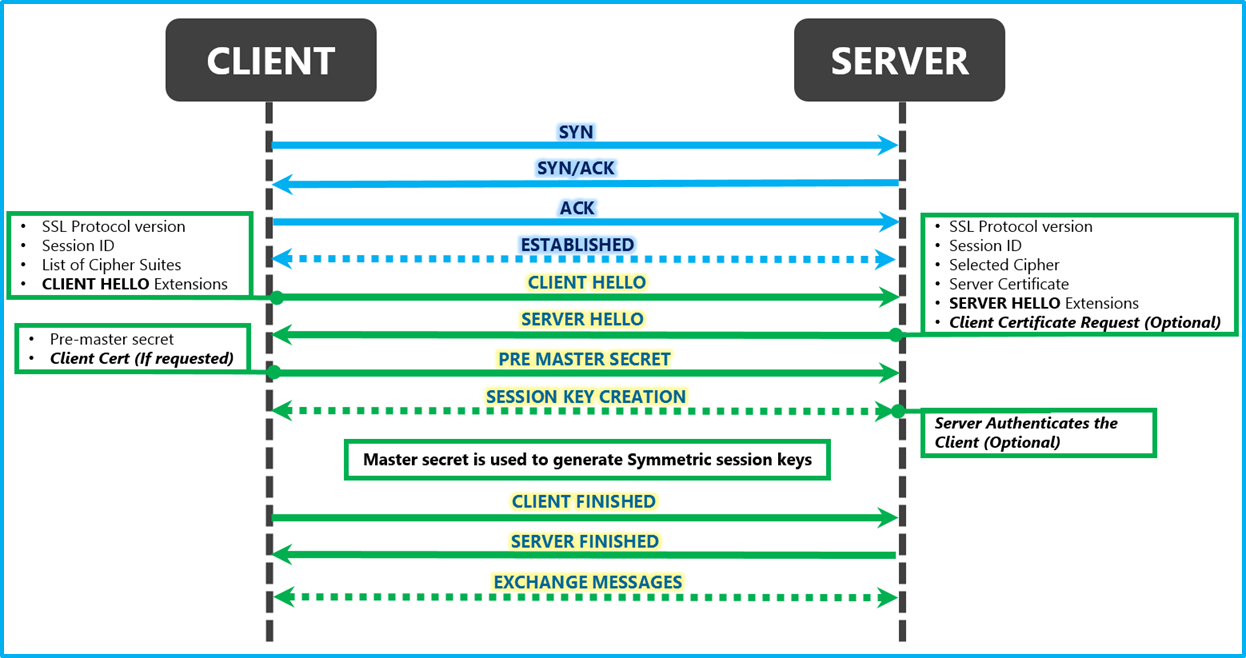
\includegraphics[width=\textwidth]{pictures/vpnVerbindungsaufbau.png}
	\caption{Verbindungsaufbau eines VPN's\cite{vanRijn2018May}}
	\label{fig:SSlhand}
\end{figure}
Die Abbildung \ref{fig:SSlhand} stellt drei Wege SSL Handshake zwischen Client und Server dar. Dabei wird zu Beginn eine unverschlüsselte Verbindung aufgebaut, indem dem Client die Server-IP und der Port mitgeteilt wird. Nachdem diese Verbindung ''ESTABLISHED'' ist, sendet der Client einen ''Client Hallo'' auf die nun bekannte IP-Adresse und den Port. Dabei liefert er das von ihm verwendete SSL Protokoll, eine Session ID, eine Liste von Chiffren, die er verwenden kann an den Server aus. Auf dieses ''Hallo'' sendet der Server selbst ein ''Server Hallo'' und liefert dabei dem Client ebenfalls seine SSL Protokoll Version, die Session ID, das von ihm gewählten Chiffre, sein Serverzertifikat und gegebenenfalls seine CCR (Client Certificate Request) aus. Hat der Client den ''Server Hallo'' erhalten, überprüft dieser die Gültigkeit, das Vertrauen in die CA und den öffentlichen Schlüssel mit der digitalen Signatur. 

Wenn er dies überprüft hat, erzeugt der Client, mit Hilfe des öffentlichen Schlüssels des Servers, ein Pre-master-secret. Dieses Secret sendet er nun an den Server. Der Server entschlüsselt das Pre-master-secret und anschließend erstellen Server und Client aus dem pre-master-secret einen symmetrischen Schlüssel, über den die Kommunikation verschlüsselt und entschlüsselt werden kann.\newline
Im Labor stießen wir auf ein nicht zu überbrückendes Hindernis. Dies entstand nach dem TCP-Handshake, im SSL-Handshake. Dabei konnte der Server sein ''Server Hallo'' nicht an den Client zurückschicken, was zur Folge hatte, dass der Client kein pre-master-secret erstellen konnte und der Vorgang abgebrochen wurde. Dieser Vorgang wurde nach 120 Sekunden erneut angestoßen und es wurde ein erneuter Verbindungsversuch unternommen, jedoch mit dem gleichen Resultat. Dieser Vorgang wird durch die Abbildung \ref{fig:logClient} und Abbildung \ref{fig:logServer} deutlich. 
\begin{figure}[h]
	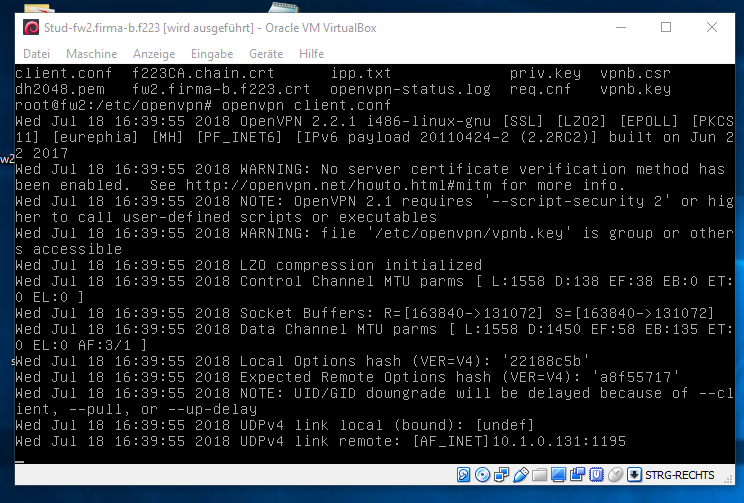
\includegraphics[width=\textwidth]{pictures/clientlog.png}
	\caption{Log Ausgabe des gestarteten VPN-Client}
	\label{fig:logClient}
\end{figure}
\begin{figure}[h]
	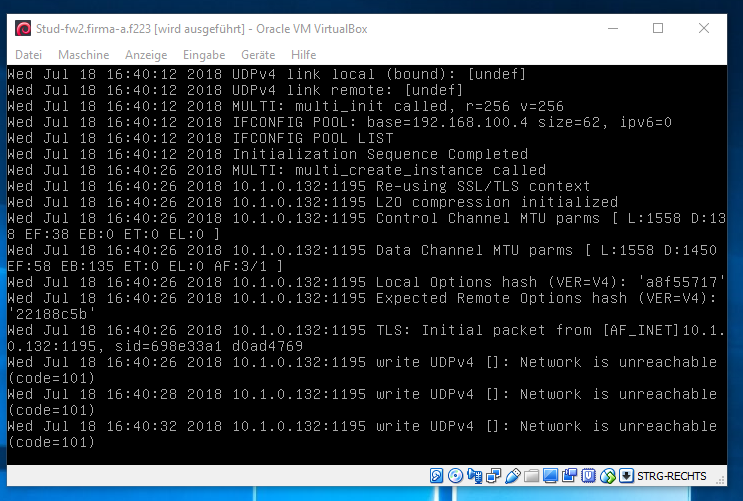
\includegraphics[width=\textwidth]{pictures/Serverlog.png}
	\caption{Log Ausgabe des gestarteten VPN-Servers}
	\label{fig:logServer}
\end{figure}
Nach Stunden der Fehlersuche und Neukonfiguration auf verschiedenen Systemen trat der Fehler erneut auf. Dies erhärtet die Vermutung, dass der Fehler in den Konfigurationen der virtuellen Maschinen zu finden sein könnte. Diese Vermutung konnte allerdings nicht bestätigt werden.  \label{Auswertung}
\section{Fazit}\label{Fazit}
Trotz der nicht gefundenen Aufklärung des Fehlers in der konfigurierten Lösung, konnten einige sehr wichtige Erkenntnisse aus diesem Praktikum gewonnen werden. Der Bereich der Netzwerkarchitektur, in Verbindung mit den vielen Sicherheitsaspekten, wird im heutigen Zeitalter immer entscheidender. Fast jeder Mitarbeiter eines globalen Unternehmens nutzt meist täglich die Möglichkeiten einer sicheren VPN-Verbindung, ohne sich darüber im Klaren zu sein, welche Komplexität bei der Bereitstellung einer solchen Verbindung überwunden werden muss. 

Nach der Absolvierung des Laborpraktikums wurden viele Aspekte, welche vorher einfach hingenommen wurden, kritisch und fachlich beleuchtet. Das Einrichten einer VPN-Verbindung mit den dazugehörigen Zertifikate, sowie die Konfiguration der internen Firewalls, bestätigt  die Annahme , dass es bei der Konfiguration von Netzwerken, auf der Basis von Linux, auf jede Kleinigkeit ankommt. So führt eine Leerzeile in einem Skript dazu, dass ein komplettes System nicht mehr so reagiert, wie es sollte. Die Schwierigkeit solch einen Fehler zu finden ist, wie das Suchen der Nadel im Heuhaufen. Zudem gestaltet sich die Fehlersuche in einem Netzwerk deutlich komplizierter, als beispielsweise in der Anwendungsentwicklung. Bei der Anwendungsentwicklung kann durch Einsatz einer IDE und dem darin enthaltenen Debugger relativ schnell auf einen Fehler geschlossen werden. Da bei der Fehlersuche eher die Gewohnheiten aus der Anwendungsentwicklung zu Grunde lagen, brauchte es etwas Zeit bis es möglich war, in dieser Domäne eine effektive und erfolgreiche Fehlersuche durchzuführen. 

Der Punkt der Fehlersuche war auch der, mit dem der größte Zeitaufwand verbunden war. Die rein logische Umsetzung der Problemstellung war relativ schnell erledigt. Auch das parallele Aufsetzen mehrerer Systeme mit dem Lösungsansatz, führte immer zum gleichen Fehlerfall, wie in der Auswertung bereits beschrieben. Selbst die intensive Hilfe der Laborassistenz konnte den Fehler nicht aufklären. Da es bei der Laborumgebung um eine virtualisierte Umgebung handelte, liegt die Vermutung nahe, dass der Fehler in der Konfiguration der virtuellen Umgebung zu finden sein könnte. Dies bleibt jedoch nur eine reine Vermutungen und konnte nicht mit Fakten belegt werden. 

Es bleibt jedoch festzuhalten, dass die Lernkurve im Rahmen des Praktikums sehr steil war. Die Bereiche der Netzwerkarchitekturen bis hin zur Erstellung eines Server-Zertifikats sind aktuell eine sehr wichtige Domäne in der Informatik. 

%%%
%%% end main document
%%%
%%%%%%%%%%%%%%%%%%%%%%%%%%%%%%%%%%%%%%%%%%%%%%%%%%%%%%%%%%%%%%%%%%%%%%%%%%%%%%%%

 \appendix %% include it, if something (bibliography, index, ...) follows below

%%%%%%%%%%%%%%%%%%%%%%%%%%%%%%%%%%%%%%%%%%%%%%%%%%%%%%%%%%%%%%%%%%%%%%%%%%%%%%%%
%%%
%%% bibliography
%%%
%%% available styles: abbrv, acm, alpha, apalike, ieeetr, plain, siam, unsrt
%%%
 \bibliographystyle{alphadin}

%%% name of the bibliography file
 \bibliography{bib/literatur.bib}

\end{document}
%%% }}}
%%% END OF FILE
%%%%%%%%%%%%%%%%%%%%%%%%%%%%%%%%%%%%%%%%%%%%%%%%%%%%%%%%%%%%%%%%%%%%%%%%%%%%%%%%
%% Local Variables:
%% mode: outline-minor
%% OPToutline-regexp: "%% .*"
%% OPTeval: (hide-body)
%% emerge-set-combine-versions-template: "%a\n%b\n"
%% End:
%% vim:foldmethod=marker
